%%%%%%%%%%%%%%%%%%%%%%%%%%%%%%%%%%%%%%%%%
% Proceedings of the National Academy of Sciences (PNAS)
% LaTeX Template
% Version 1.0 (19/5/13)
%
% This template has been downloaded from:
% http://www.LaTeXTemplates.com
%
% Original author:
% The PNAStwo class was created and is owned by PNAS:
% http://www.pnas.org/site/authors/LaTex.xhtml
% This template has been modified from the blank PNAS template to include
% examples of how to insert content and drastically change commenting. The
% structural integrity is maintained as in the original blank template.
%
% Original header:
%% PNAStmpl.tex
%% Template file to use for PNAS articles prepared in LaTeX
%% Version: Apr 14, 2008
%
%%%%%%%%%%%%%%%%%%%%%%%%%%%%%%%%%%%%%%%%%

%----------------------------------------------------------------------------------------
%	PACKAGES AND OTHER DOCUMENT CONFIGURATIONS
%----------------------------------------------------------------------------------------

%------------------------------------------------
% BASIC CLASS FILE
%------------------------------------------------

%% PNAStwo for two column articles is called by default.
%% Uncomment PNASone for single column articles. One column class
%% and style files are available upon request from pnas@nas.edu.

%\documentclass{pnasone}
\documentclass{pnastwo}

%------------------------------------------------
% POSITION OF TEXT
%------------------------------------------------

%% Changing position of text on physical page:
%% Since not all printers position
%% the printed page in the same place on the physical page,
%% you can change the position yourself here, if you need to:

% \advance\voffset -.5in % Minus dimension will raise the printed page on the 
                         %  physical page; positive dimension will lower it.

%% You may set the dimension to the size that you need.

%------------------------------------------------
% GRAPHICS STYLE FILE
%------------------------------------------------

%% Requires graphics style file (graphicx.sty), used for inserting
%% .eps/image files into LaTeX articles.
%% Note that inclusion of .eps files is for your reference only;
%% when submitting to PNAS please submit figures separately.

%% Type into the square brackets the name of the driver program 
%% that you are using. If you don't know, try dvips, which is the
%% most common PC driver, or textures for the Mac. These are the options:

% [dvips], [xdvi], [dvipdf], [dvipdfm], [dvipdfmx], [pdftex], [dvipsone],
% [dviwindo], [emtex], [dviwin], [pctexps], [pctexwin], [pctexhp], [pctex32],
% [truetex], [tcidvi], [vtex], [oztex], [textures], [xetex]

\usepackage{graphicx}

%------------------------------------------------
% OPTIONAL POSTSCRIPT FONT FILES
%------------------------------------------------

%% PostScript font files: You may need to edit the PNASoneF.sty
%% or PNAStwoF.sty file to make the font names match those on your system. 
%% Alternatively, you can leave the font style file commands commented out
%% and typeset your article using the default Computer Modern 
%% fonts (recommended). If accepted, your article will be typeset
%% at PNAS using PostScript fonts.

% Choose PNASoneF for one column; PNAStwoF for two column:
%\usepackage{PNASoneF}
%\usepackage{PNAStwoF}

%------------------------------------------------
% ADDITIONAL OPTIONAL STYLE FILES
%------------------------------------------------

%% The AMS math files are commonly used to gain access to useful features
%% like extended math fonts and math commands.

\usepackage{amssymb,amsfonts,amsmath}

%------------------------------------------------
% OPTIONAL MACRO FILES
%------------------------------------------------

%% Insert self-defined macros here.
%% \newcommand definitions are recommended; \def definitions are supported

%\newcommand{\mfrac}[2]{\frac{\displaystyle #1}{\displaystyle #2}}
%\def\s{\sigma}

%------------------------------------------------
% DO NOT EDIT THIS SECTION
%------------------------------------------------

%% For PNAS Only:
% \contributor{Submitted to Proceedings of the National Academy of Sciences of the United States of America}
% \url{www.pnas.org/cgi/doi/10.1073/pnas.0709640104}
% \copyrightyear{2008}
% \issuedate{Issue Date}
% \volume{Volume}
% \issuenumber{Issue Number}

%----------------------------------------------------------------------------------------

\begin{document}

%----------------------------------------------------------------------------------------
%	TITLE AND AUTHORS
%----------------------------------------------------------------------------------------

\title{Contact prediction workflow using Snakemake} % For titles, only capitalize the first letter

%------------------------------------------------

%% Enter authors via the \author command.  
%% Use \affil to define affiliations.
%% (Leave no spaces between author name and \affil command)

%% Note that the \thanks{} command has been disabled in favor of
%% a generic, reserved space for PNAS publication footnotes.

%% \author{<author name>
%% \affil{<number>}{<Institution>}} One number for each institution.
%% The same number should be used for authors that
%% are affiliated with the same institution, after the first time
%% only the number is needed, ie, \affil{number}{text}, \affil{number}{}
%% Then, before last author ...
%% \and
%% \author{<author name>
%% \affil{<number>}{}}

%% For example, assuming Garcia and Sonnery are both affiliated with
%% Universidad de Murcia:
%% \author{Roberta Graff\affil{1}{University of Cambridge, Cambridge,
%% United Kingdom},
%% Javier de Ruiz Garcia\affil{2}{Universidad de Murcia, Bioquimica y Biologia
%% Molecular, Murcia, Spain}, \and Franklin Sonnery\affil{2}{}}

\author{John Lamb\affil{1}{Stockholm University, SciLife Lab}}

\contributor{Submitted for the Applied Bioinformatics course, as part of the MedBioInfo graduate school}

%----------------------------------------------------------------------------------------

\maketitle % The \maketitle command is necessary to build the title page

\begin{article}

%----------------------------------------------------------------------------------------
%	ABSTRACT, KEYWORDS AND ABBREVIATIONS
%----------------------------------------------------------------------------------------

\begin{abstract}
Here we present a snakemake pipeline for automatically making contact predictions from a protein sequence. It comes
    bundled with \textit{jackhmmer} as an aligner and \textit{ccmpred} as a contact predictor. This is fully modularized
    and can easily be changed to preference. 
    The workflow is set up to take full advantage of the underlying hardware and will automatically use the available
    cores and run potential steps in parallell to increase speed of execution.
\end{abstract}

%------------------------------------------------

\keywords{contact prediction | workflow | snakemake} % When adding keywords, separate each term with a straight line: |

%------------------------------------------------

%% Optional for entering abbreviations, separate the abbreviation from
%% its definition with a comma, separate each pair with a semicolon:
%% for example:
%% \abbreviations{SAM, self-assembled monolayer; OTS,
%% octadecyltrichlorosilane}

% \abbreviations{}
% \abbreviations{SAM, self-assembled monolayer; OTS, octadecyltrichlorosilane}

%----------------------------------------------------------------------------------------
%	PUBLICATION CONTENT
%----------------------------------------------------------------------------------------

%% The first letter of the article should be drop cap: \dropcap{} e.g.,
%\dropcap{I}n this article we study the evolution of ''almost-sharp'' fronts

\section{Introduction}

\dropcap{R}unning a contact prediction pipeline from a protein sequence is usually conducted as a multi-step process.
    Multiple intermittent files are created and running a full dataset of samples requires special attention to create
    code that make full use of the underlying hardware. 
    To simplify this we have used snakemake to create a scaleable and modular pipeline to run contact predictions from
    sequence.
    Snakemake is a workflow management system built to create reproducible and scalable data pipelines. Workflows are
    described in a human readable, Python based, format. 
    %It is easily scaled and can be seamlessly deployed to servers
    %or clusters without any changes to the workflow. In addition, it can be fully selfcontained and include a
    %describtion of the required software and automatically deploy this into an executioin environment.

%----------------------------------------------------------------------------------------
%	MATERIALS AND METHODS
%----------------------------------------------------------------------------------------

%% Optional Materials and Methods Section
%% The Materials and Methods section header will be added automatically.

\begin{materials}
    The workflow has been divided up in several modules that each handle one single part, see figure \ref{dag}. Each
    sample first go through the alignment-module where the samples are aligned, by default, using
    \textit{jackhmmer}
    against a database. The result of this is then fed into the convert-module that converts the output from the aligner
    to correct format for the chosen predictor. The predictor is by default \textit{ccmpred} and the result from these
    predictions are fed into the extract-module that extract the top couplings for each sample. All of the samples are
    then collected into a summary report from which the topcouplings of each sample is accessable. 
\begin{figure}[h]
\centerline{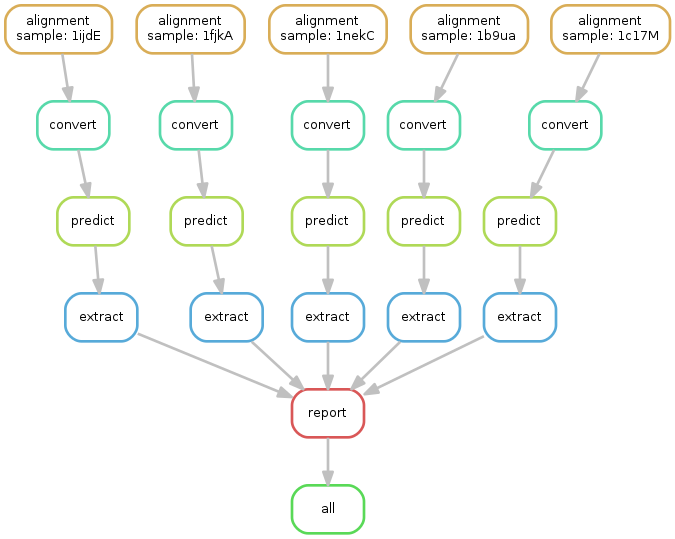
\includegraphics[width=1.0\linewidth]{dag.png}}
\caption{Workflow schematic with five samples}\label{dag}
\end{figure}
    An important part for scalability is that each module can be specified to use a certain number of cores. Snakemake
    will automatically try to saturate the available cores so will automatically run modules in parallell if possible.
    This can clearly be seen when this workflow is run as the alignment-module by default takes the maximum number of
    cores available and hence the samples are all run in sequence. However, the rest of the modules can only utilise one
    single core and snakemake will then automatically run these modules in parallell. This does extend to later modules
    as well so if some samples has finished the convert-module they to not have to wait for the other samples to finish
    the same module but can progress to the predict-module given there are cores available. This is only true if there
    are no interdependencies between the samples. The report-module will always wait until all extract-modules has run
    as it is dependent on all samples having finished.

    To make the workflow as modularized as possible each module consists of a separate driver script that runs the
    underlying code or chosen program. By minimizing the parameters to mostly only input and output directories the
    choice of program running each module is easily changed. Each driver script is written to return to \textbf{stdout}
    which is then easily captured by snakemake. This means that a change of underlying aligner or predictor is done by a
    change of call signature in each modules driver script.

    All configurations are made in the config.yaml file that specifices input/output directories, database for alignment
    and any potential limitation on how many cores to use. Snakemake will automatically scale down the number of cores
    to maximum of available cores.
    The path to the input directory and the path to the local database file are usually the only two options that needs
    to be set.
    The workflow with by default create a results directory in the running directory for all output and the number of
    cores are set to use all available. 
    
\end{materials}
\section{Results}

The workflow is fully modularized and deployable and works out of the box with the bundled jackhmmer and ccmpred. By
creating a virtual Python3 environment and pip install requirements according to the requirements file and adjusting the
database file path to a local database the five test samples run and creates a result folder in the current working
directory. This contains all intermediate files together with a summarized report. If these intermediate files are not
essential snakemake has an easy feature to stamp intermittend files as temporary and will automatically clean these up.
This however will make these files regenerated every time the workflow is run which is not always the wanted result.
%------------------------------------------------

\section{Discussion}

Snakemake is proven to be a good framework for workflows. It does require some rethinking in the way it functions but as
it is similar in principle to GNU make it can quickly be picked up by anyone that has used make before. Even without
previous experience it is easy to learn but require a more bottoms-up approach to the workflow than the traditional
top-down.
A next step in this project is full integration with a running environment and/or container. Snakemake has support for
automatic deployment using conda and virtual environment and also to archive fully contained workflows into tarballs for
full reproducibility.

As snakemake rules are connected throught the respective input and output files any type of workflow can be generalized.
With the use of dummy files any type of directed acyclic workflow could be defined and be run in optimal order and
potetial steps be run in parallell automatically handled by snakemakes without the user having to specify anything more
than available cores.
%%%%%    Snakemake is proven to be a good framework for workflows. It does require some rethinking in the way it functions but as
%%%%%    it is similar in principle to GNU make it can quickly be picked up by anyone that has used make before. Even without
%%%%%    previous experience it is easy to learn but require a more bottoms-up approach to the workflow than the traditional
%%%%%    top-down.
%%%%%    A next step in this project is full integration with a running environment and/or container. Snakemake has support for
%%%%%    automatic deployment using conda and virtual environment and also to archive fully contained workflows into tarballs for
%%%%%   full reproducibility.
%----------------------------------------------------------------------------------------
%	ACKNOWLEDGEMENTS
%----------------------------------------------------------------------------------------

%----------------------------------------------------------------------------------------
%	BIBLIOGRAPHY
%----------------------------------------------------------------------------------------

%% PNAS does not support submission of supporting .tex files such as BibTeX.
%% Instead all references must be included in the article .tex document. 
%% If you currently use BibTeX, your bibliography is formed because the 
%% command \verb+\bibliography{}+ brings the <filename>.bbl file into your
%% .tex document. To conform to PNAS requirements, copy the reference listings
%% from your .bbl file and add them to the article .tex file, using the
%% bibliography environment described above.  

%%  Contact pnas@nas.edu if you need assistance with your
%%  bibliography.

% Sample bibliography item in PNAS format:
%% \bibitem{in-text reference} comma-separated author names up to 5,
%% for more than 5 authors use first author last name et al. (year published)
%% article title  {\it Journal Name} volume #: start page-end page.
%% ie,
% \bibitem{Neuhaus} Neuhaus J-M, Sitcher L, Meins F, Jr, Boller T (1991) 
% A short C-terminal sequence is necessary and sufficient for the
% targeting of chitinases to the plant vacuole. 
% {\it Proc Natl Acad Sci USA} 88:10362-10366.


%% Enter the largest bibliography number in the facing curly brackets
%% following \begin{thebibliography}
\begin{thebibliography}{10}
\bibitem{snakemake}
K\"oster,~Johannes and Rahman,~Sven, {\em Snakemake - A scalable bioinformatics workflow engine}, Bioinformatics, (2012).
\bibitem{jackhmmer}
R.D.~Finn et al., {\em HMMER Web Server: 2015 update}, Nucleic Acids Research,  Web Server Issue 43 (2015), W30--W38.
\bibitem{ccmpred}
Seemayer~S, Gruber~M, S\"oding~J., {\em CCMpred -- fast and precise prediction of protein residue-residue contacts from
        correlated mutations}, Bioinformatics, 30 (2014), pp.~3128--3130
\bibitem{improvedcontact}
Skwark~MJ, Raimond~D, Michel~M, Elofsson~A, {\em Improved Contact Predictions Using the Recognition
        of Protein Like Contact Patterns}, PLOS Comput Biol, (2014), e1003889
\bibitem{structpred}
Michel~M, Men\'endez~Hurtado~D, Uziela~K, Elofsson~A, {\em Large-scale structure prediction by improved contact
        predictions and model quality assessment.}, Bioinformatics, 33 (2017), pp.~23--29
\end{thebibliography}
% \begin{acknowledgments}
% This work was partially supported by a grant from the Spanish Ministry of Science and Technology.
% \end{acknowledgments}

%----------------------------------------------------------------------------------------
%	BIBLIOGRAPHY
%----------------------------------------------------------------------------------------

%% PNAS does not support submission of supporting .tex files such as BibTeX.
%% Instead all references must be included in the article .tex document. 
%% If you currently use BibTeX, your bibliography is formed because the 
%% command \verb+\bibliography{}+ brings the <filename>.bbl file into your
%% .tex document. To conform to PNAS requirements, copy the reference listings
%% from your .bbl file and add them to the article .tex file, using the
%% bibliography environment described above.  

%%  Contact pnas@nas.edu if you need assistance with your
%%  bibliography.

% Sample bibliography item in PNAS format:
%% \bibitem{in-text reference} comma-separated author names up to 5,
%% for more than 5 authors use first author last name et al. (year published)
%% article title  {\it Journal Name} volume #: start page-end page.
%% ie,
% \bibitem{Neuhaus} Neuhaus J-M, Sitcher L, Meins F, Jr, Boller T (1991) 
% A short C-terminal sequence is necessary and sufficient for the
% targeting of chitinases to the plant vacuole. 
% {\it Proc Natl Acad Sci USA} 88:10362-10366.


%% Enter the largest bibliography number in the facing curly brackets
%% following \begin{thebibliography}


%------------------------------------------------
\end{article}

%----------------------------------------------------------------------------------------
%	FIGURES AND TABLES
%----------------------------------------------------------------------------------------

%% Adding Figure and Table References
%% Be sure to add figures and tables after \end{article}
%% and before \end{document}

%% For figures, put the caption below the illustration.
%%
%% \begin{figure}
%% \caption{Almost Sharp Front}\label{afoto}
%% \end{figure}

%%%%% \begin{figure}[h]
%%%%% \centerline{
\includegraphics[width=0.4\linewidth]{placeholder.jpg}}
%%%%% \caption{Figure caption}\label{placeholder}
%%%%% \end{figure}

%% For Tables, put caption above table
%%
%% Table caption should start with a capital letter, continue with lower case
%% and not have a period at the end
%% Using @{\vrule height ?? depth ?? width0pt} in the tabular preamble will
%% keep that much space between every line in the table.

%% \begin{table}
%% \caption{Repeat length of longer allele by age of onset class}
%% \begin{tabular}{@{\vrule height 10.5pt depth4pt  width0pt}lrcccc}
%% table text
%% \end{tabular}
%% \end{table}

%----------------------------------------------------------------------------------------

\end{document}
